\documentclass[11pt]{beamer}

% From sybila preamble
% https://github.com/sybila/presentation-template/blob/master/presentation.tex
\usetheme[progressbar=frametitle]{metropolis}
\usepackage{appendixnumberbeamer}

\usepackage[utf8]{inputenc}

\usepackage{booktabs}
\usepackage[scale=2]{ccicons}

\usepackage{pgfplots}
\usepgfplotslibrary{dateplot}

\usepackage{xspace}
\newcommand{\themename}{\textbf{\textsc{metropolis}}\xspace}
\definecolor{mSybilaRed}{HTML}{990000}

\setbeamercolor{title separator}{
  fg=mSybilaRed
}

\setbeamercolor{progress bar}{%
  fg=mSybilaRed,
  bg=mSybilaRed!90!black!30
}

\setbeamercolor{progress bar in section page}{
  use=progress bar,
  parent=progress bar
}

\setbeamercolor{alerted text}{%
  fg=mSybilaRed
}

% End of sybila styling


% Using Gonzolo's answer here https://tex.stackexchange.com/questions/105613/footer-in-beamer
%   to provide a way of numbering
\setbeamertemplate{footline}
{%
  \leavevmode%
  \hbox{\begin{beamercolorbox}[wd=.5\paperwidth,ht=2.5ex,dp=1.125ex,leftskip=.3cm,rightskip=.3cm]{author in head/foot}%
  % Added by me, includes buttons on every slide
  \vspace{10pt}\hyperlinkslideprev{\beamerreturnbutton{prev}}
  \hyperlinkslidenext{\beamergotobutton{next}}
  \end{beamercolorbox}%
  \begin{beamercolorbox}[wd=.5\paperwidth,ht=2.5ex,dp=1.125ex,leftskip=.3cm,rightskip=.3cm plus1fil]{author in head/foot}%
    \usebeamerfont{author in head/foot}\insertshortauthor\hfill\insertpagenumber
  \end{beamercolorbox}}%
  \vskip0pt%
}



\usepackage{wrapfig}
\usepackage{tikz}
\usepackage{pgfplots}
\usepackage{pgfplotstable}
\pgfplotsset{compat=1.18}

\usepackage{bookmark}

\hypersetup{
    colorlinks = true,
}


\title{MENG 330}
\subtitle{Project Two}
\author{Lucas Johnston}
\date{\today}


\begin{document}
    \maketitle
   
    % Add to PDF indices
    % Will need to manually update if adding more pages
    \bookmark[page=1,level=0]{Title Slide}
    \bookmark[page=2,level=0]{The Part}
    \bookmark[page=3,level=0]{Supports and Loads}
    \bookmark[page=3,level=1]{Supports}
    \bookmark[page=4,level=1]{Loads}
    \bookmark[page=5,level=0]{Mesh Sizing}
    \bookmark[page=6,level=0]{Convergence Results}
    \bookmark[page=7,level=0]{Material Properties}
    \bookmark[page=8,level=0]{Results}
    \bookmark[page=8,level=1]{Image}
    \bookmark[page=9,level=1]{Comparison}
    \bookmark[page=10,level=0]{Error Sources}
    \bookmark[page=10,level=1]{General Setup}
    \bookmark[page=11,level=1]{Convergence}

    
    \begin{frame}{The Part}
        \begin{itemize}
            \item Steel shaft with 18 lbf and 32 lbf gear loads applied (not shown) 
        \end{itemize}

        \begin{figure}[H]
            \centering
            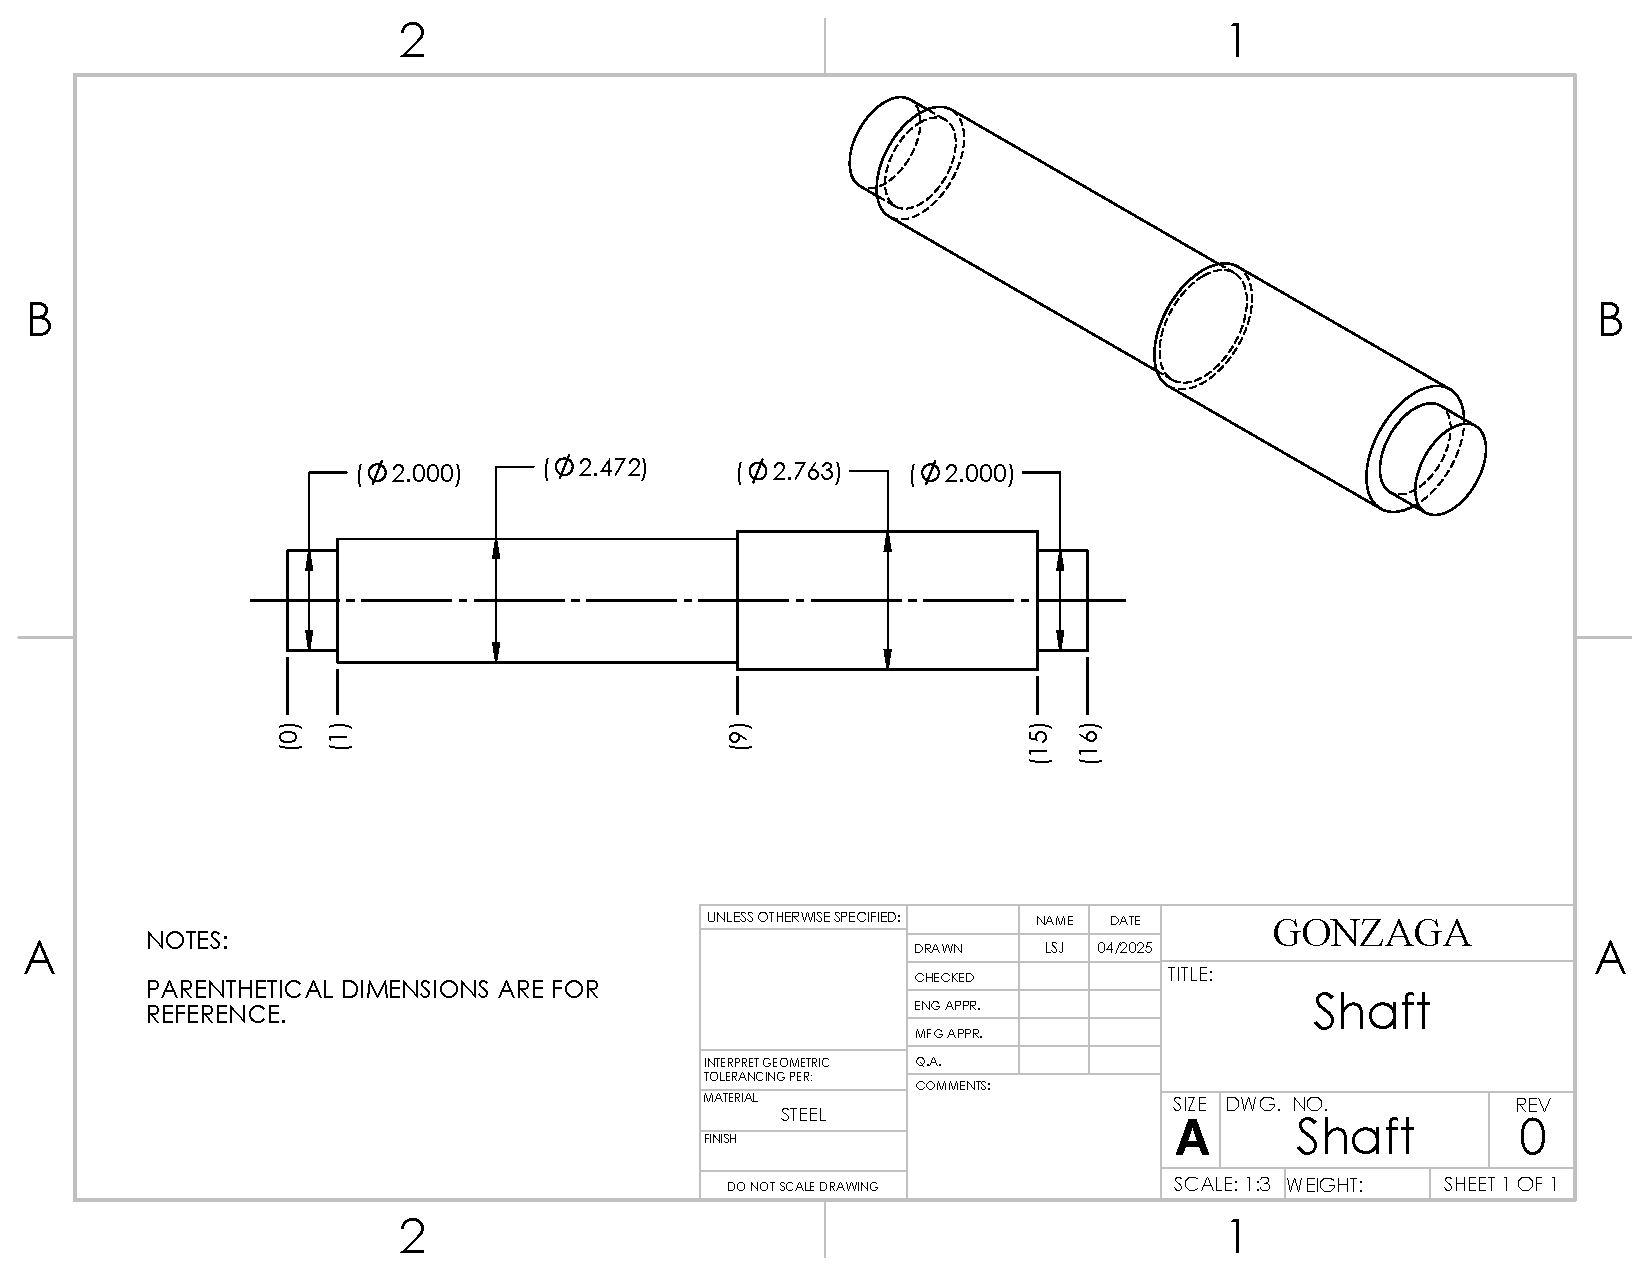
\includegraphics[height=0.60\textwidth]{figs/Shaft.pdf}
        \end{figure}
    \end{frame}

    \begin{frame}{Supports and Loads: Supports}
        \begin{itemize}
            \item Two bearing reactions
            \item Modeled as remote displacement boundary conditions
                \begin{itemize}
                    \item Right support fixed position in y,z, free in x, free rotation in x,y,z
                    \item Left support fixed position in x,y,z, free rotation in y,z
                        \begin{itemize} 
                            \item Results didn't change if rotation fixed in x or not
                        \end{itemize}
                \end{itemize}
        \end{itemize}
        \begin{figure}
            \centering
            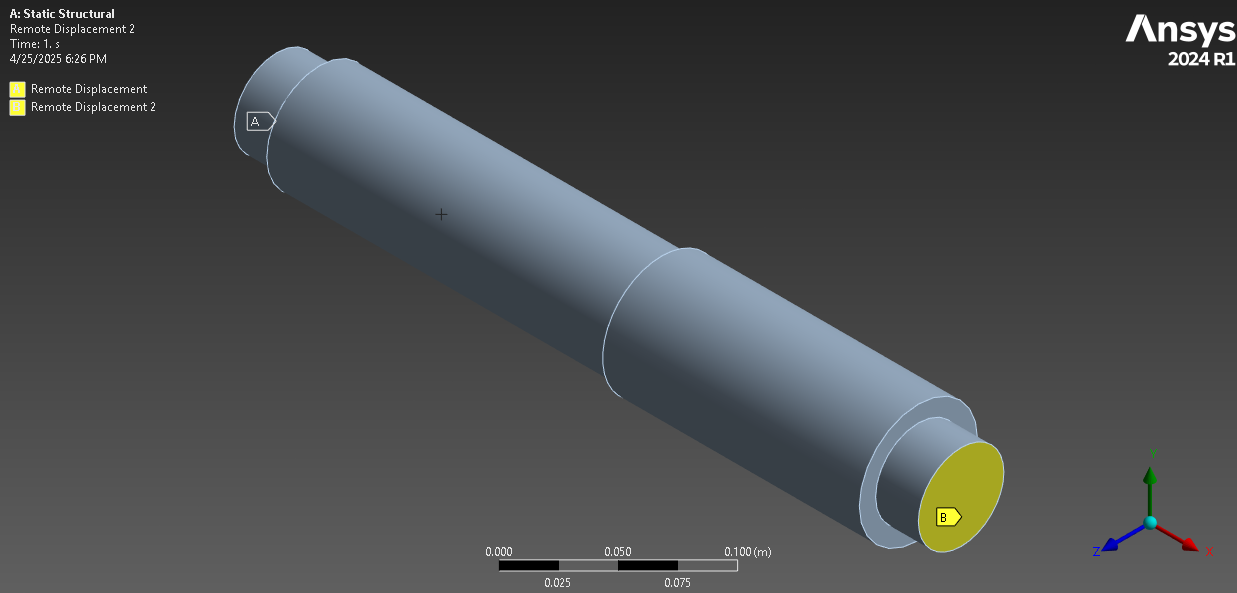
\includegraphics[scale=0.22]{figs/BC_all_iso.png}
            \caption{Loading Conditions}
        \end{figure}
    \end{frame}

    \begin{frame}{Supports and Loads: Loads}
        \begin{itemize}
            \item Used remote displacement to place loads in center of beam at given distance
                \begin{itemize} 
                    \item Adding cutout geometry to apply load to resulted in crushing, larger deflections
                \end{itemize}
            \item External forces, convert to metric
                \begin{itemize}
                    \item $ 18 \textrm{ lbf} \approx 80.068 \textrm{ N}  $
                    \item $ 32 \textrm{ lbf} \approx 142.343 \textrm{ N} $
                \end{itemize}
        \end{itemize}
        \begin{figure}
            \centering
            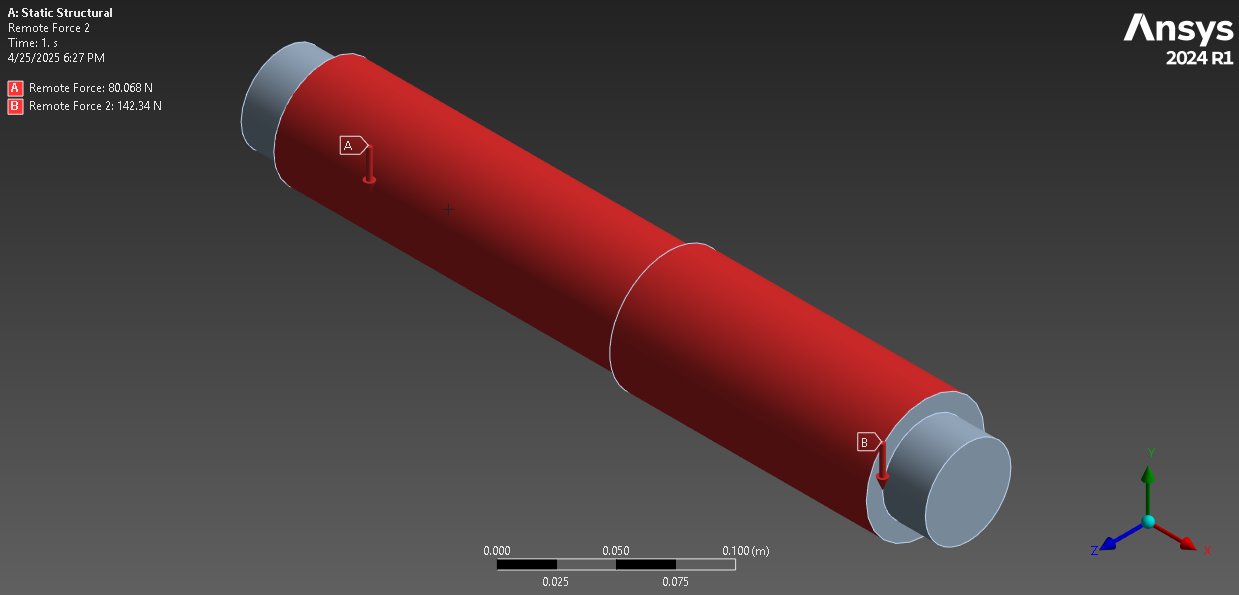
\includegraphics[scale=0.20]{figs/forces_iso.png}
            \caption{Loading Conditions}
        \end{figure}
    \end{frame}


    \begin{frame}{Mesh Sizing}
       \begin{itemize} 
            \item Used automatic option for meshing (used triangles)
            \item Decided to use 5e-3 m element size for all of body
            \item No further refinement was used
        \end{itemize}

        \vspace{10pt}
        \begin{figure}[H]
            \centering
            \vspace{-17pt}
            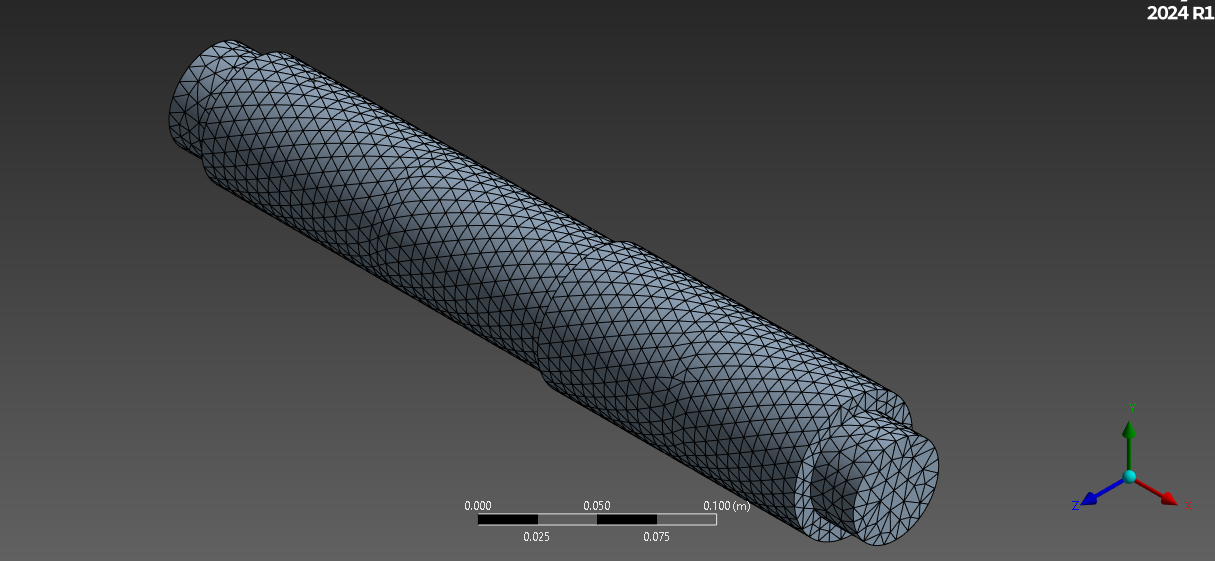
\includegraphics[scale=0.215]{figs/mesh_iso.png}
            % \vspace{-20pt}
            \caption{Mesh}
        \end{figure}
    \end{frame}

    \begin{frame}{Convergence Results} 
        \begin{itemize}
            \item Had $\approx50\%$ error for 7.5e-3 m element size for all of body
            \item Settled on 5e-3 m element size for all of body for better accuracy
            \item Did not use additional refinement
        \end{itemize}
        \vspace{10pt}
        \begin{figure}[H]
            \centering
            \vspace{-17pt}
            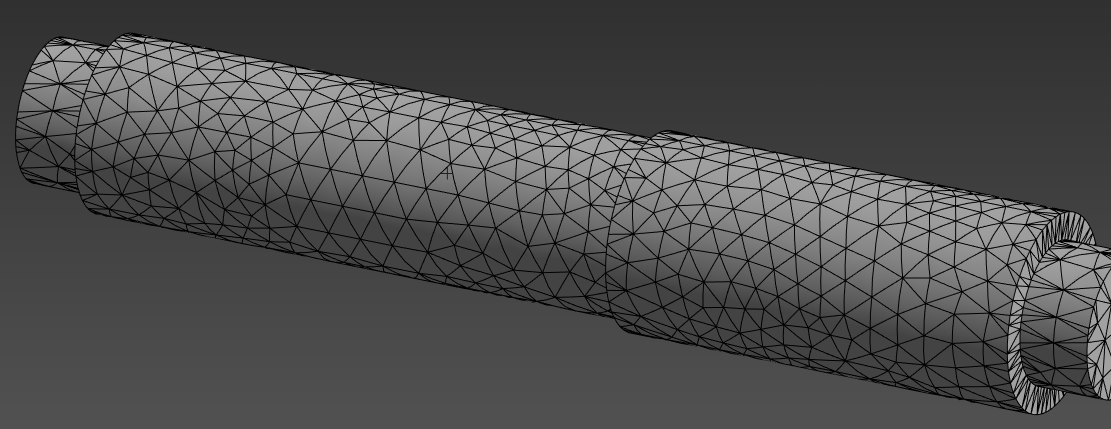
\includegraphics[scale=0.215]{figs/old_mesh_coarse_cropped.png}
            % \vspace{-20pt}
            \caption{7.5e-3 m Element Size Mesh}
        \end{figure}
    \end{frame}

    % \begin{frame}{Analyzed Results: Step Response}
    %     \begin{table}[!ht]
    %         \scalebox{0.60}{
    %             \centering
    %             \begin{tabular}{|l|l|l|l|}
    %             \hline
    %                 \textbf{Time (s)} & \textbf{Load (N)} & \textbf{Stress (Pa)} & \textbf{Deflection (m/m)} \\
    %                 \hline\hline
    %                 1 & 50 & 7.47990E+06 & 3.74120E-05 \\ \hline
    %                 2 & 100 & 7.46090E+06 & 3.73170E-05 \\ \hline
    %                 3 & 200 & 7.44510E+06 & 3.72380E-05 \\ \hline
    %                 4 & 400 & 7.50240E+06 & 3.75250E-05 \\ \hline
    %             \end{tabular}
    %         }
    %         \caption{Stress, Strain Response to Changing Force}
    %     \end{table}
    %     \begin{figure}[H]
    %         \vspace{-15pt}
    %         \begin{tikzpicture}[scale=0.6]
    %             \begin{axis}[
    %                     xlabel =Load (N),
    %                     ylabel =Stress (Pa),
    %                 ]
    %                 \addplot
    %                 %table[y=Stress_Pa, x=Load_N, col sep=comma]{figs/loading_steps_table_no_spaces.csv}
    %                 % This is the loading steps table, I just modified a Min Working Example to 
    %                 %   get it to match
    %                 table[x=LoadN,y=StressPa,col sep=comma] {figs/table.csv}; 
    %             \end{axis}
    %         \end{tikzpicture}
    %         \vspace{-15pt}
    %         \caption{Stress vs. Load}
    %         \label{fig:stress_v_load}
    %     \end{figure}
    % \end{frame}

    % \begin{frame}{Analyzed Results: Analytical Values}
    %     \begin{itemize} 
    %         \item Have analytical solution for stress at top element of wall
    %         \item Use this value to validate FEA model
    %         \begin{equation}
    %             \sigma_{\textrm{eq}} = \sqrt{\frac{{\left(\sigma_1 - \sigma_2\right)}^2 + {\left(\sigma_2 - \sigma_3\right)}^2 + {\left(\sigma_3 - \sigma_1\right)}^2}{2}}
    %         \end{equation}
    %         \item Apply principle stresses solution from \href{https://github.com/A-Person7/a_design_class/blob/main/hw3/problem1.m}{here}
    %         \begin{equation}\label{analytic_sln}
    %             \hspace{-24pt}
    %             \resizebox{1\textwidth}{!}{$%
    %                 \sigma_{\textrm{eq}} = \sqrt{\frac{{\left(24.488\textrm{ MPa} - 0\textrm{ MPa}\right)}^2 + {\left(0\textrm{ MPa} - -929.903\textrm{ MPa}\right)}^2 + {\left(-929.903\textrm{ MPa} - 24.488\textrm{ MPa}\right)}^2}{2}} \approx 942.39\textrm{ MPa}
    %             $%
    %             }%
    %         \end{equation}
    %         \item Now have a way to check if Ansys simulation converges to sensical value
    %     \end{itemize}
    % \end{frame}

    % \begin{frame}{Analyzed Results: Computational and Analytical Comparison}
    %     \begin{itemize} 
    %         \item Saw within 1.5\% of expected theoretical value 
    %         \begin{itemize}
    %             \item see Table \ref{tab:meshsizes}
    %         \end{itemize}
    %         \item Simulation consistently underestimated stress
    %         \item Simulation reported maximum stress at `crook' of beam elbow joint
    %         \begin{itemize} 
    %             \item Have no analytical values there to compare to
    %         \end{itemize}
    %     \end{itemize}
    % \end{frame}

    % \begin{frame}{Sources of Error}
    %     \begin{itemize} 
    %         \item Most likely source of error is lack of mesh refinement
    %         \begin{itemize}
    %             \item Didn't specifically refine mesh around elbow joint
    %             \item Saw very high expected stress values at joint, higher than would expect
    %             \item Suggests that elbow joint mesh could be refined for better results
    %         \end{itemize}
    %         \item Should also check for discrepancies between loading conditions (e.g. force acting at centroid or at edge)
    %     \end{itemize}

    %     \begin{figure} 
    %         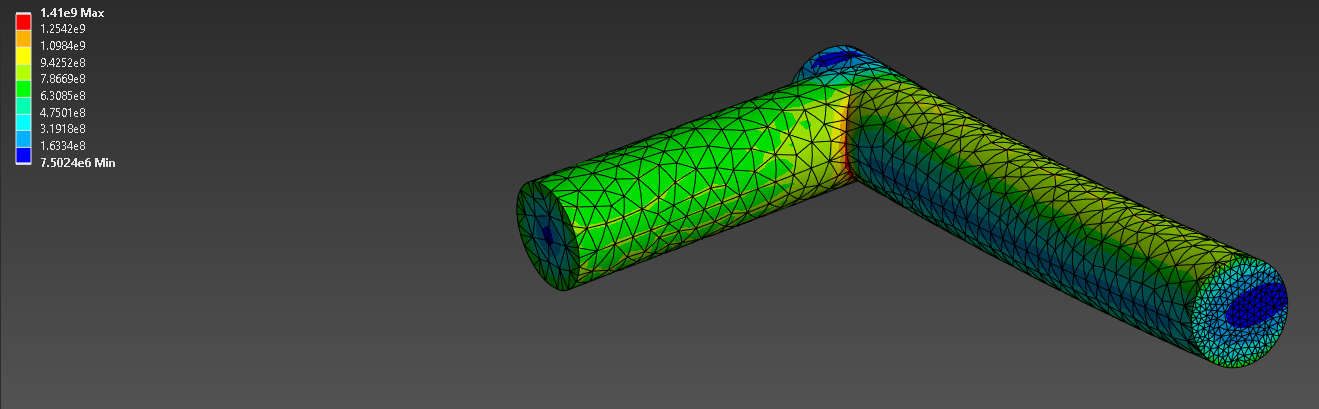
\includegraphics[scale=0.25]{figs/3E-3_Body_1E-3_Face/von_mises_eq_stress_better_view_cropped.png}
    %         \vspace{-7pt}
    %         \caption{Computed Stress at Elbow Joint (stress in units of Pa)}
    %     \end{figure}
    % \end{frame}


    \begin{frame}{Material Properties}
        \begin{itemize}
            \item Structural Steel (Ansys material library)
            \item Evaluated at 22\textdegree\ Celcius
            \item Chosen as it's a typical material for this application
        \end{itemize}
        \begin{table}
            \scalebox{0.8}{
                \begin{tabular}{|c|c|c|} 
                    \hline
                    \textbf{Property} & \textbf{Value} & \textbf{Unit} \\
                    \hline\hline
                    Young's Modulus & 2E+11 & Pa\\ 
                    \hline
                    Poisson's Ratio & 0.3 &  \\
                    \hline
                    Bulk Modulus & 1.6667E+11 & Pa\\
                    \hline
                    Shear Modulus & 7.6223E+10 & Pa\\
                    \hline
                \end{tabular}
            }
            \caption{Structural Steel Properties}\label{tab:mat}
        \end{table}
    \end{frame}

    \begin{frame}{Results: Image}
       \begin{itemize} 
            \item Result of Ansys simulation 
            \item Probes added to nearest mesh location of points of interest
        \end{itemize}

        \vspace{10pt}
        \begin{figure}[H]
            \centering
            \vspace{-17pt}
            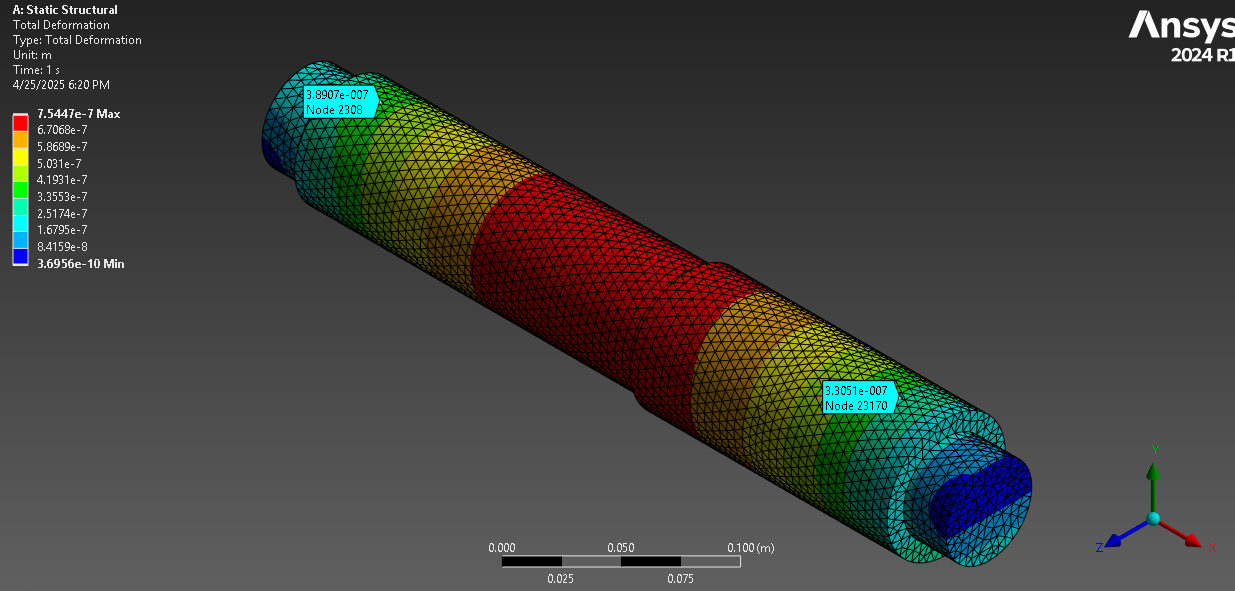
\includegraphics[scale=0.215]{figs/deflection_iso.png}
            % \vspace{-20pt}
            \caption{Mesh}
        \end{figure}
    \end{frame}

    \begin{frame}{Results: Comparison}
        \begin{itemize}
            \item My \href{https://github.com/A-Person7/a_design_class/blob/main/hw7/problem3.m}{MATLAB code} predicts the following deflections:
            \begin{itemize} 
                \item Remove semicolons at the end of lines 80, 81, displayed results in inches, left and right deflections respectively
                \item Left deflection $1.0456\cdot10^{-05} \textrm{ in} \approx 2.655824\cdot10^{-7} \textrm{ m}$
                \item Right deflection $1.0067\cdot10^{-05} \textrm{ in} \approx 2.557018\cdot10^{-7} \textrm{ m}$
            \end{itemize}
        \end{itemize}

        \begin{table}[!ht]
            \centering
            \begin{tabular}{|l|l|l|l|}
            \hline
                ~ & ANSYS [$10^{-7}$ m] & MATLAB [$10^{-7}$ m] & \% Difference \\ \hline
                Left & 3.8907 & 2.655824 & 37.73\% \\ \hline
                Right & 3.3051 & 2.557018 & 25.52\% \\ \hline
            \end{tabular}
            \caption{Deflection Comparison}
        \end{table}
    \end{frame}


    \begin{frame}{Error sources: General Setup}
        \begin{itemize}
            \item Young's Modulus differed slightly between MATLAB and ANSYS simulations 
                \begin{itemize} 
                    \item Young's Modulus in \href{https://canvas.gonzaga.edu/courses/18311/files/folder/Additional\%20Content?preview=4057043}{\texttt{ShaftDeflectionEnglish.m}} is $30\cdot 10^{6}$ psi
                    \item Young's Modulus in ANSYS simulation is listed as $2\cdot10^{11}$ Pa (see Table \autoref{tab:mat})
                        \begin{itemize}
                            \item $2\cdot10^{11}$ Pa $\approx 28\textrm{,}007\textrm{,}550$ psi
                        \end{itemize}
                    \item Inherently introduces an $\approx 3.5$\% error
                \end{itemize}
            \item \textbf{Boundary Conditions are likely the most influential error}
                \begin{itemize} 
                    \item \textbf{Bearing boundary conditions likely culprit}, hard to model simply supported beam
                    \item Load boundary conditions were essentially identical to theoretical case (stick load on simply supported beam would have loads acting in the center)
                \end{itemize}
        \end{itemize}
    \end{frame}

    \begin{frame}{Error sources: Convergence}
        \begin{itemize}
            \item ANSYS shaft may have not had enough elements for this setup to converge more
                \begin{itemize} 
                    \item Saw better results going from $7.5\cdot10^{-5}$ m $\to$ $5\cdot10^{-5}$ m, but didn't use smaller sizes as it took too long
                    \item Could have also used refinement around shoulder faces
                \end{itemize}
            \item Did not expiriment much with other meshing types
                \begin{itemize} 
                    \item Might have observed closer values with other element types
                \end{itemize}
            \item \texttt{ShaftDeflectionEnglish.m} might have used different numerical integration scheme
                \begin{itemize}
                    \item \texttt{ShaftDeflectionEnglish.m} uses \href{https://www.mathworks.com/help/matlab/ref/cumtrapz.html}{cumtrapz}, a trapezoidal numerical integration method
                \end{itemize}
        \end{itemize}
    \end{frame}
\end{document}
